\chapter{$Q$-clouds}
\label{ch:Q}

\epigraph{``\emph{
Ask veit eg standa, \\
heitir Yggdrasill, \\
hár baðmur, ausinn \\
hvíta auri; \\
þaðan koma döggvar \\
þær er í dala falla, \\
stendur æ yfir grænn \\
Urðarbrunni. 
} 
''}{19th verse of Völuspá}
%%%%%%%%%%%%%%%%%%%%%%%%%%%%%%%%%%%%%%%%%%%%%%%%%%%%%%%%%%%%%%%%%%%%%%%%%%%%%%%
\section{Introduction}

$Q$-balls are complex scalar field solitons, obtained with a non-renormalizable self-interaction, arising in some effective field theories. 
These non-topological solitons circumvent the standard Derrick-type argument~\cite{Derrick:1964ww} by virtue of having a
time-dependent phase for the scalar field.
The global phase-invariance of the scalar field theory leads to a conserved Noether
charge $Q$, corresponding to particle number.
Such configurations have a rich structure and
found a variety
of physically interesting applications;
for example, they appear in supersymmetric generalizations of the standard model \cite{Kusenko:1997zq}, 
and have been suggested to generate baryon number or to be dark matter candidates~\cite{Kusenko:1997si}.

\bigskip

Here, we report that $Q$-balls can become $Q$-clouds, when replacing the near (Minkowski) origin region with a black hole horizon\footnote{
Boson shells harbouring black holes have been studied in \cite{Kleihaus:2010ep}.
However, these solutions require a V-shaped scalar potential which
is not of the form (\ref{QU}).}.
This fits into a general pattern observed in soliton physics~\cite{Bizon:1994dh,Volkov:1998cc,Herdeiro:2014ima}; for the case discussed herein, however, the black hole \textit{must rotate}, by virtue of condition (\ref{super_cond}), and the scalar field's frequency is closely related to the rotation of the black hole.
The relation between the scalar field's parameters and the horizon angular velocity can actually be seen as a \textit {rotation synchronization condition}, as discussed in \cite{Benone:2014ssa}. 
%
%
%%%%%%%%%%%%%%%%%%%%%%%%%%%%%%%%%%%%%%%%%%%%%%%%%%%%%%%%%%%%%%%%%%
\section{The model}
%%%%%%%%%%%%%%%%%%%%%%%%%%%%%%%%%%%%%%%%%%%%%%%%%%%%%%%%%%%%%%%%%%



We consider the action for a complex scalar field with a self-interaction potential $U(\left| \Phi \right|)$:
\begin{equation}
\label{Qaction}
S=-\int \left[ 
   \frac{1}{2} g^{\mu\nu}\left( \Phi_{, \, \mu}^* \Phi_{, \, \nu} + \Phi _
{, \, \nu}^* \Phi _{, \, \mu} \right) + U( \left| \Phi \right|) 
 \right] \sqrt{-g} d^4x
\ . 
\end{equation}
A usual choice for the potential in the $Q$-ball literature is 
\begin{equation}
U(|\Phi|) =  \mu^2 |\Phi|^2-\lambda |\Phi|^4 +\beta |\Phi|^6,
\label{QU} 
\end{equation}
with $\mu$ being the boson mass and $\lambda,\beta>0$.
This potential is chosen such that non-topological soliton solutions
exist in a flat spacetime background, see $e.g.$ the discussion in \cite{Volkov:2002aj}.

Variation of Eq. \eqref{Qaction} with respect to the scalar field
leads to the non-linear Klein-Gordon equation,
\begin{equation}
\label{KG}
 \Box\Phi= \frac{\partial U}{\partial\left|\Phi\right|^2}\Phi \ ,
\end{equation}
where $\Box$ represents the covariant d'Alembert operator.
%
%
The stress-energy tensor $T_{\mu\nu}$ of the scalar field is
\begin{eqnarray}
T_{\mu \nu} 
=  \Phi_{, \, \mu}^*\Phi_{, \, \nu}
+\Phi_{, \, \nu}^*\Phi_{, \, \mu} -g_{\mu\nu} \left[ \frac{g^{\alpha\beta} }{2} 
\left( \Phi_{, \, \alpha}^*\Phi_{, \, \beta}+
\Phi_{, \, \beta}^*\Phi_{, \, \alpha} \right)+U(|\Phi|)\right]
 \ .
\label{tmunu} 
\end{eqnarray}

For the background metric,
we consider a general 
ansatz with two Killing vectors   $\xi=\partial_t$ and $\eta=\partial_\varphi$ (with $t$ and $\varphi$
the time and azimuthal coordinates, respectively),
which in an appropriate coordinate system
can be written as
\begin{eqnarray}
\label{metric-ansatz}
ds^2= g_{rr}dr^2+g_{\theta \theta} d\theta^2 +g_{\varphi\varphi}d\varphi^2+2 g_{\varphi t}d\varphi dt +g_{tt} dt^2 \ .
\end{eqnarray}
$g_{\mu\nu}$ 
are functions of the spherical coordinates $r$ and $\theta$ only. We assume asymptotic flatness. Thus, as $r\to \infty$, $g_{rr} \to 1$,
$g_{\theta \theta} \to r^2$,
$g_{\varphi\varphi} \to r^2\sin^2 \theta$,
$g_{\varphi t} \to 0$
and
$g_{tt} \to -1$.
We also assume the existence of an event horizon, located
at a constant value of $r=r_H$.
This 
is a Killing horizon of the Killing vector field
$\chi=\xi+\Omega_H \eta$,
where $\Omega_H$ is computed as
\begin{eqnarray}
\label{OmegaH}
\Omega_H=-\frac{\xi^2}{\xi \cdot \eta}\bigg |_{r_H}=-\frac{g_{tt}}{g_{t\varphi}}\bigg |_{r_H}.
\end{eqnarray}

The scalar field ansatz is of the form of Eq. \eqref{eqn:field-ansatz}, 
 where $\phi$ is a real function, $w>0$ is the frequency and $m=\pm 1,\pm 2$\dots
is the azimuthal harmonic index. 
As was discussed in the introduction, the $(t, \varphi)$-dependences of $\Phi$ occur as phase factors only.
This implies that $T_{\mu\nu}$ is $(t, \varphi)$-independent, which is required for
a configuration to be stationary and axisymmetric.
The energy-momentum tensor, however,  will 
 depend on both $m$ and $w$.

With the ansatz Eq. \eqref{eqn:field-ansatz}, (\ref{metric-ansatz}), 
the Klein-Gordon equation Eq. \eqref{KG}
reduces to
\begin{eqnarray}
\label{KG1}
\frac{1}{\sqrt{-g}}\frac{\partial}{\partial r}\left(g^{rr}\sqrt{-g}\frac{\partial \phi}{\partial r} \right)+
\frac{1}{\sqrt{-g}}\frac{\partial}{\partial \theta} \left(g^{\theta \theta}\sqrt{-g}\frac{\partial \phi}{\partial \theta} \right)
\nonumber\\
-\left(
m^2 g^{\varphi \varphi}-2g^{\varphi t} +w^2 g^{tt} 
\right)\phi
=(\mu^2-2 \lambda \phi^2+3\beta \phi^4)\phi.~{~}
\end{eqnarray}
We are interested in 
localized, particle-like solutions of this equation,
 with a finite scalar amplitude $\phi$ and a regular energy density distribution.
These axially symmetric configurations carry a nonzero 
  mass-energy and angular momentum,  which are defined as
\begin{eqnarray}
\label{scalar-charges}
E=-2\pi \int_{r_H}^\infty dr \int_0^\pi d\theta \sqrt{-g}T_t^t\ , \qquad 
J= 2\pi \int_{r_H}^\infty dr \int_0^\pi d\theta \sqrt{-g}T_\varphi^t \ .
 \end{eqnarray}
%
Moreover, a conserved charge $Q$ exists, associated with the complex scalar field $\Phi$, since the Lagrange density is invariant under the global phase transformation
$\Phi \to \Phi e^{i\alpha}$, 
 leading to the conserved current
 \begin{eqnarray}
\label{scalar-current}
j^{\mu}=-i\left[\Phi^* \partial^\mu\Phi+\Phi \partial^\mu\Phi^*\right]\ , \qquad \nabla_\mu j^{\mu}=0 \ .
 \end{eqnarray}
The corresponding conserved charge $Q$ is the integral of $j^t$ on spacelike slices.
One can easily see that in the absence of backreaction the following relation holds:
 \begin{eqnarray}
\label{rel1}
J=m Q\ ,
\end{eqnarray}
such that  angular momentum  is quantized.
Moreover,
in view of this relation, the spinning solutions
can be thought as corresponding to minima of energy with fixed angular
momentum.
 
 
In our approach, $Q$-clouds are found by solving the Klein-Gordon equation Eq. \eqref{KG1}
with suitable boundary conditions.  
Then the energy and angular momentum are computed
from the numerical output.
The boundary conditions result from the study of the solutions
on the boundary of the integration domain. 
The behavior of the scalar field as $r\to \infty$ must agree
with linear analysis: $\phi=f(\theta)  {e^{-\sqrt{\mu^2-w^2}r}}/{r}+\dots$;
thus $\phi|_{r=\infty}$=0, while the existence of a bound state requires $w <\mu $.
Axial symmetry and
regularity impose that the scalar field vanishes on the symmetry axis ($\theta=0,\pi$).
At the horizon, we suppose the existence of a power series expansion of the scalar field,
of the form
\begin{eqnarray}
\label{scalar-horizon}
\phi(r,\theta)=\phi_{0}( \theta)+\phi_{1}( \theta)(r-r_H)+\phi_{2}( \theta)(r-r_H)^2+\dots,
\end{eqnarray}
with finite coefficients $\phi_{k}$.
%
It turns out that, supposing $\phi_{0}\neq 0$, such an expansion holds if and only if condition \eqref{super_cond} holds. 
Thus, the synchronization condition is required by regularity and not only as a consequence of obtaining clouds.
After replacing Eq. \eqref{scalar-horizon} into the Klein-Gordon equation, one obtains an involved condition between the coefficients
$\phi_{0}$, $\phi_{1}$ and $\phi_{2}$ 
which should be satisfied at $r=r_H$.
The explicit form of this condition depends on the coordinate system one chooses to work with,
and shall be discussed below.

 

%%%%%%%%%%%%%%%%%%%%%%%%%%%%%%%%%%%%%%%%%%%%%%%%%%%%%%%%%%%%%%%%%%
\section{The solutions}
%%%%%%%%%%%%%%%%%%%%%%%%%%%%%%%%%%%%%%%%%%%%%%%%%%%%%%%%%%%%%%%%%%

 
Similarly to previous works 
\cite{Volkov:2002aj,Kleihaus:2005me}, 
the  numerical solutions reported here have been found for 
the following parameters in 
the potential
defined by Eq. \eqref{QU}:
%
\begin{equation}
\lambda = 2,~~\beta=1,~~\mu^2=1.1~.
\label{param}
\end{equation} 
But solutions with other choices of $\lambda,\beta$
have also been considered.
%
In particular, preliminary results indicate that the constraints
on the potential $U$  required
for the existence of flat space $Q$-balls~\cite{Coleman:1985ki}, 
also hold for the black hole background. 
%
Let us also remark that,
for given $(\mu,w,m)$,
solutions with other values of $\lambda$, $\beta$
can be generated by using the scaling symmetry
\begin{equation}
\phi^{(\lambda_2,\beta_2)}=\sqrt{\frac{\lambda_1}{\lambda_2}}\phi^{(\lambda_1,\beta_1)},~~
E^{(\lambda_2,\beta_2)}=\frac{\lambda_1}{\lambda_2}E^{(\lambda_1,\beta_1)},~~Q^{(\lambda_2,\beta_2)}=\frac{\lambda_1}{\lambda_2}Q^{(\lambda_1,\beta_1)},~~
{\rm with}~~\beta_2=\frac{\lambda_2^2}{\lambda_1}.
\label{symm}
\end{equation} 

All quantities and variables of interest are expressed in natural units set by the scalar field mass $\mu$.

The $Q$-clouds discussed here are invariant under a reflection along  
the equatorial plane; these are commonly referred to, in this context, as \textit{even parity solutions}. Odd parity
solutions, on the other hand, should also exist, and their $Q$-ball limit has been considered in 
\cite{Volkov:2002aj,Kleihaus:2007vk}.

Finally, here we focus on a Kerr black hole background, but similar solutions are likely to exist on any spinning black hole.

%%%%%%%%%%%%%%%%%%%%%%%%%%%%%%%%%%%%%%%%%%%%%%%%%%%%%%%%%%%%%%%%%%
\subsection{Limiting known cases: flat space $Q$-balls and Kerr linear clouds}
%%%%%%%%%%%%%%%%%%%%%%%%%%%%%%%%%%%%%%%%%%%%%%%%%%%%%%%%%%%%%%%%%% 



$Q$-clouds have two known limiting cases: (i) flat space $Q$-balls and (ii) Kerr linear clouds. We shall now briefly review some relevant properties of both these cases which are of interest to understand $Q$-clouds. 

\bigskip


Spinning $Q$-balls have been constructed  in 
\cite{Volkov:2002aj,Kleihaus:2005me};
a review of their properties can be found in \cite{Radu:2008pp}.
%
One imposes that the scalar field
vanishes at the origin, in a spherical coordinate system,  $\phi|_{r=0}=0$, which is implied by demanding regularity of the energy density.
Treating $w,m$ and the parameters in the potential $U$
as input variables, $Q$-balls 
exist only in a certain frequency range, 
$w_{min} < w < w_{max}=\mu$.
An estimate for $w_{min}$
is given by the condition 
\cite{Volkov:2002aj,Kleihaus:2005me}
\begin{eqnarray}
 w_{min}^2\sim  {\rm min} [U(\phi)/\phi^2]=\mu^2-\frac{\lambda^2}{4\beta}<w^2,
\end{eqnarray}
even though this limit could not be reached for spinning solutions.
%
At a critical value of the frequency in the interval $]w_{min}, w_{max}[$, 
both the $Q$-balls' mass-energy and angular momentum attain their minimum value,
from where they monotonically increase towards both limiting values
of the frequency.
%
Thus, considering the $Q$-ball's mass as a function of their Noether charge $Q$,
there are two branches of solutions, merging and ending
at the minimal charge and mass. 
$Q$-balls are stable along (most of) the lower frequency branch~\cite{Radu:2008pp},
where their mass is smaller than the mass of $Q$ free bosons.
%
Concerning their spatial distribution, for a given frequency, 
the amplitude $\phi(r,\theta)$, energy-momentum and charge
densities are maximal on the equatorial plane and the energy is concentrated in a toroidal
region encircling the symmetry-axis.

The limiting behaviour of the spinning $Q$-balls near the boundaries of the allowed frequency interval
is rather intricate, and has not yet been discussed in a systematic way  in the literature. 
It appears that 
both $E$ and $Q$
increase without bound at the limits of the $w$-interval, even though these limits are difficult to investigate.
Also, $Q$-balls become large there in terms of their spatial distribution;
as $w\to w_{min}$,
they can be viewed as squashed spheroids, homogeneously filled inside.
For $w\to w_{max}$, the solutions
also become large spheroids, but this time they are hollow, with the maximal energy density
concentrated at the surface and being close to zero everywhere else.  

\bigskip
  
A very different picture has been found in~\cite{Herdeiro:2014goa,Benone:2014ssa}
for the simpler case of a non-self-interacting
scalar field
on a fixed Kerr black hole background.
These linear scalar clouds
satisfy the same boundary conditions as stated above.
However, their study is  simpler, since in this case
the Klein-Gordon equation admits separation of variables. 
%
Then the problem reduces to solving
an ordinary differential equation for 
the radial function $R_{nlm}(r)$.
This has been done in~\cite{Herdeiro:2014goa,Benone:2014ssa} and determines the position of the existence lines for a cloud with quantum numbers $(n,l,m)$. Three examples of these lines are exhibited in Fig. \ref{existencelines}, in a mass ($M$) vs. horizon angular velocity ($\Omega_H$) diagram for Kerr black holes.
%
Analytical estimates for these lines have been found in 
\cite{Hod:2012px,Hod:2013zza}
for the case of a (nearly-)extremal Kerr black hole.


\begin{figure}[h!]
\centering
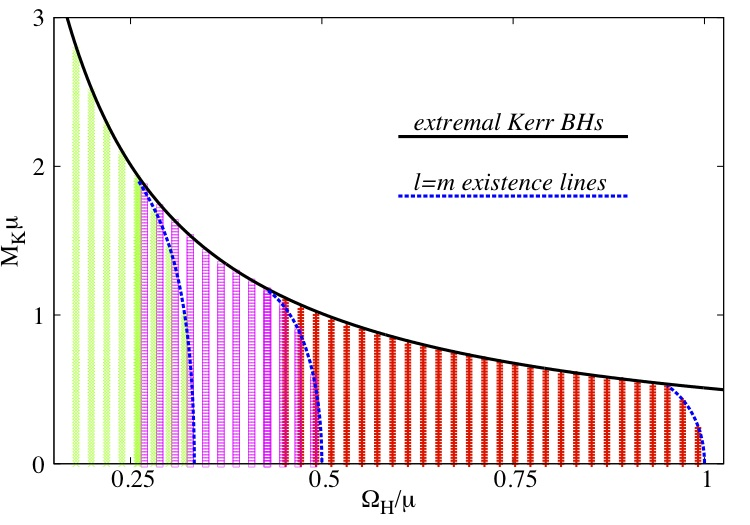
\includegraphics[height=2.8in]{papers/QClouds/Mw.jpeg}
\caption{Existence (blue dotted) lines with $n=0$, $m=l=1,2,3$, from right to left, respectively, for linear clouds on the Kerr background.  Kerr black holes exist below the solid black line, which corresponds to extremal Kerr solutions. For each $m$, $\Omega_H^{extremal}$ is the value of $\Omega_H$ at which the corresponding existence line intersects the curve of extremal black holes. The (vertical sets of) filling points in the diagram correspond to examples of $Q$-cloud solutions with $m=1$ (red/dark grey), $m=2$ (purple/medium grey) and $m=3$ (green/light grey). $Q$-clouds with a given value of $m$ exist between the existence line for linear clouds with $n=0$, $m=l$ and a minimal frequency.} 
\label{existencelines}
\end{figure}

The existence line with $n=0$ and $l=m$ divides the Kerr parameter space in two regions. To the left (right) of the line stand the Kerr backgrounds which are superradiantly stable (unstable) against scalar field perturbations with azimuthal harmonic index $m$.


%%%%%%%%%%%%%%%%%%%%%%%%%%%%%%%%%%%%%%%%%%%%%%%%%%%%%%%%%%%%%%%%%%
\subsection{Non-linear $Q$-clouds on the Kerr black hole background}
%%%%%%%%%%%%%%%%%%%%%%%%%%%%%%%%%%%%%%%%%%%%%%%%%%%%%%%%%%%%%%%%%%

When turning on the scalar field self-interactions in the potential, i.e. giving them a small but non-zero value, the non-linearities prevent a separation of variables, similar to the one discussed above. 
For given $(w,m)$,
the scalar field $\phi$ is a superposition of
spheroidal harmonics, whose amplitudes, however, differ from $R_{nlm}(r)$.
Then following \cite{Volkov:2002aj}, one can write
% 
\begin{eqnarray}
\phi(r,\theta)=\sum_{k=0}^\infty f_k(r)S_{m+2k,m} (\theta),
\end{eqnarray}
%
which results in an infinite set of ordinary differential
equations for $f_k(r)$.
In principle, this set can be truncated for some $k_{max}$
and then solved numerically.
In our approach, however, we have chosen to solve
 directly the partial differential equation (\ref{KG1}). But instead of using Boyer-Lindquist coordinates -- 
 which yield a complicated boundary condition at  $r=r_H$,  in terms of the scalar function and its first and second derivatives -- we have used quasi-isotropic coordinates for Kerr (see e.g.~\cite{Cook:2000vr}).  In parallel, a large set of solutions have been computed  by using a radially shifted version of the Boyer-Lindquist coordinate system, for which $r\to r-\frac{a^2}{r_H}$.
%
Both these coordinate systems yield a near horizon expansion for the scalar field, defined in Eq. \eqref{scalar-horizon}, with the $\phi_1$ term absent, thus allowing us to impose a standard Neumann boundary condition there.
                                                                
  
Our central result in this chapter is
that {\it all flat space Q-ball solutions can be generalized to Q-clouds on a Kerr black hole background}.
The black hole parameters, however, are not arbitrary, as implied by condition (\ref{super_cond}).
%
%
The solutions are found by starting with a flat spacetime
configuration with given $(w,m)$ and increasing the size of the black hole
(as given $e.g.$ by the event horizon area)
via the parameter $r_H$.  
We have constructed in a systematic way solutions with $m=1,2,3$ (around 20000 solutions for each case). A subset of the solutions for each of these values of $m$ has been plotted in Fig.~\ref{existencelines}.  When varying the horizon size, there are two 
possible behaviours for the solutions with a given $w$: 
\begin{itemize}
\item[(i)]

For $m\Omega_H^{extremal}/\mu\leq w/\mu <1$,  $Q$-clouds start from flat spacetime $Q$-balls (i.e. with zero horizon size)
 and end on the existence line for linear clouds with $n=0$, $l=m$. The value of $\Omega_H^{extremal}$ depends on $m$; for instance,  $\Omega_H^{extremal}\simeq 0.95,0.43,0.26$  for $m=1,2,3$, respectively (see $e.g.$~\cite{Hod:2013zza}). As the existence line is approached,
the amplitude of the scalar field amplitude 
decreases to zero and 
the linear scalar clouds are recovered.
 
\item[(ii)]
For  $m\Omega_H^{min}\leq w <m\Omega_H^{extremal}$,
any Kerr black hole with $\Omega_H=w/m$ is allowed as a background for a $Q$-cloud solution.
In particular, one finds scalar clouds also on extremal Kerr black holes,
which provide one boundary for the domain of existence. Again, the value of $\Omega_H^{min}$ depends on $m$ and they seem to coincide, in terms of $w_{min}$, with the corresponding value for $Q$-balls.
%

\end{itemize}
%
The bottom line is that $Q$-clouds exist between the $l=m$, $n=0$ existence line for linear clouds and a minimal frequency/horizon angular velocity -- Fig. \ref{existencelines}. A number of configurations with $m=4,5$
have also been found;
thus we expect their existence for any $m\geq 1$.

A generic $Q$-cloud solution has nonzero mass and angular momentum,
with a toroidal distribution for the corresponding densities -- Fig. \ref{densities}.
% 
The scalar profile looks rather similar to that known in the flat spacetime limit
(with the region $r<r_H$ removed from it).
Note, however, that similarly to the behaviour observed for linear scalar clouds~\cite{Benone:2014ssa}, 
the scalar field amplitude does not vanish at the horizon,
approaching its maximum on the equatorial plane.
The energy density $-T_t^t$
vanishes on the symmetry axis, except for $m=1$ solutions.


\begin{figure}[h!]
\centering
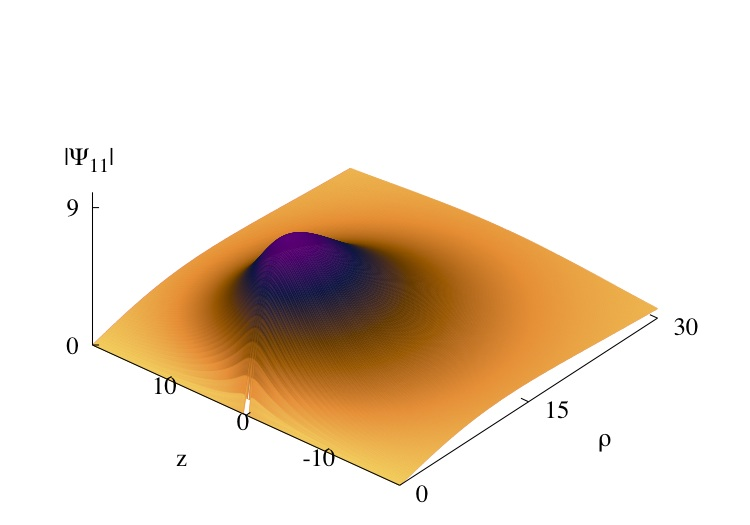
\includegraphics[height=2.2in]{papers/QClouds/Z-3d.jpeg}
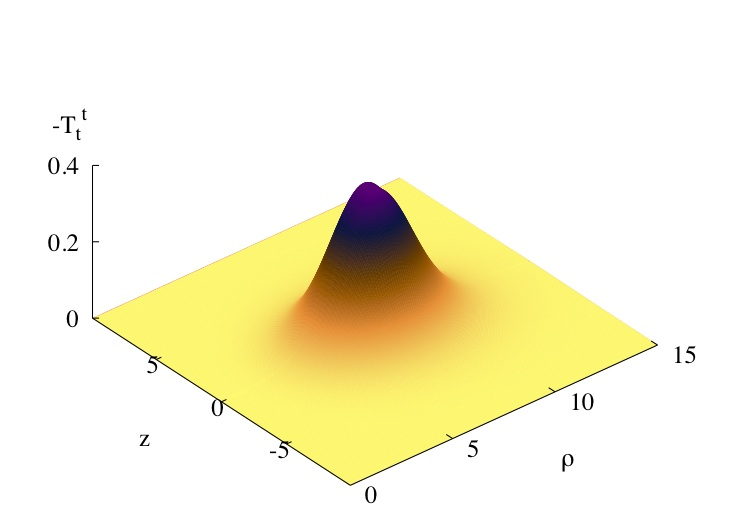
\includegraphics[height=2.2in]{papers/QClouds/E-3d.jpeg}
\caption{The scalar field and the energy density are shown for a typical
 non-linear $Q$-cloud with $m=2$, $w =1$ (in terms of `polar' coordinates $\rho=r\sin \theta$,
 $z=r \cos \theta$).
The Kerr black hole background has an event horizon radius (in quasi-isotropic coordinates) at
 $r_H=0.03$. 
} 
\label{densities}
\end{figure}

In Fig. \ref{energy1}, we plot the energy 
of $Q$-clouds as a function of several parameters of the Kerr black hole background. These results have been obtained for $m=1$, but a similar picture has been found for $m=2,3$. A similar pattern is observed for the angular momentum $J$.

\begin{figure}[h!]
\centering
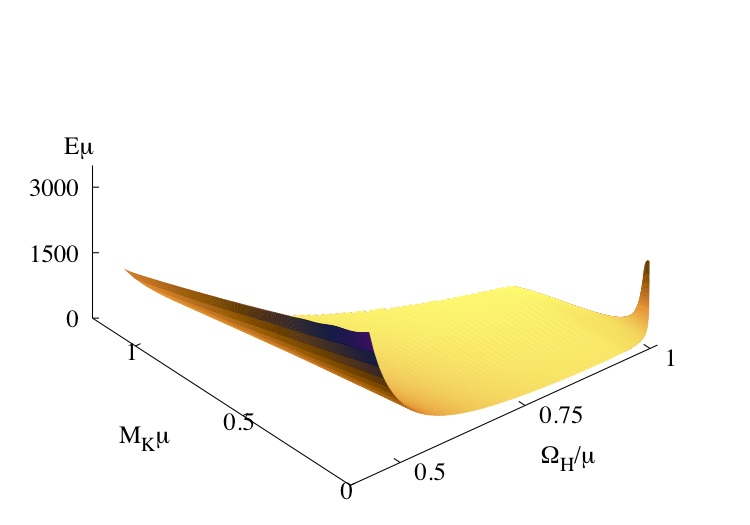
\includegraphics[height=2.15in]{papers/QClouds/EMw-3D.jpeg}
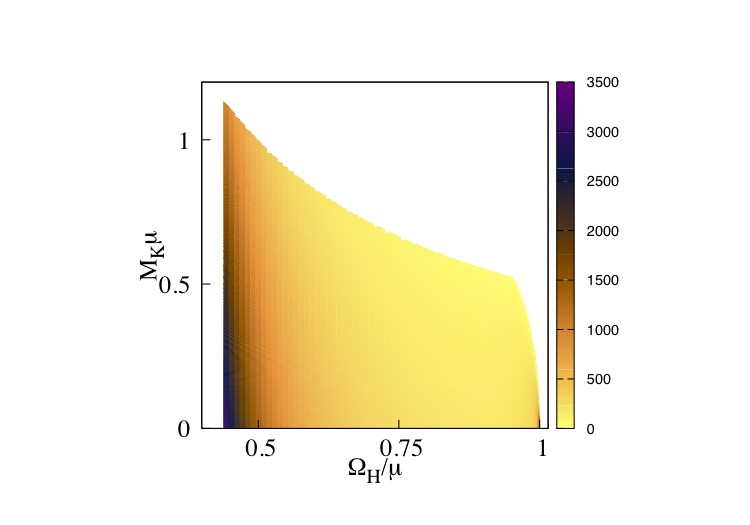
\includegraphics[height=2.15in]{papers/QClouds/EMw-2D.jpeg}
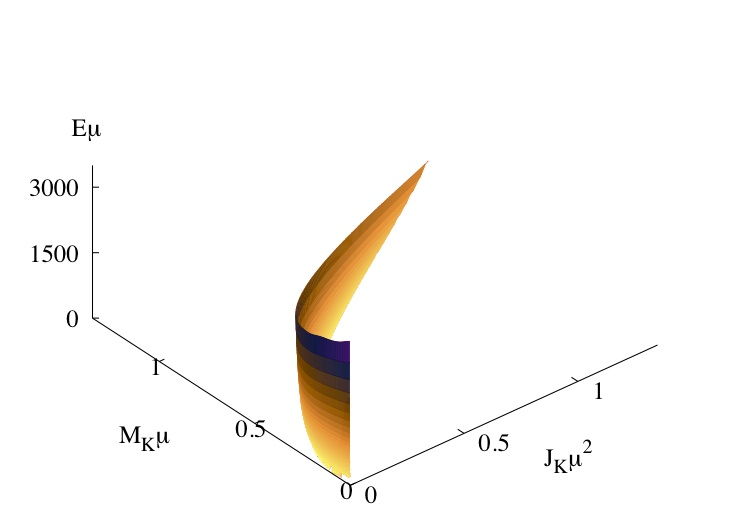
\includegraphics[height=2.15in]{papers/QClouds/EMJ-3D.jpeg}
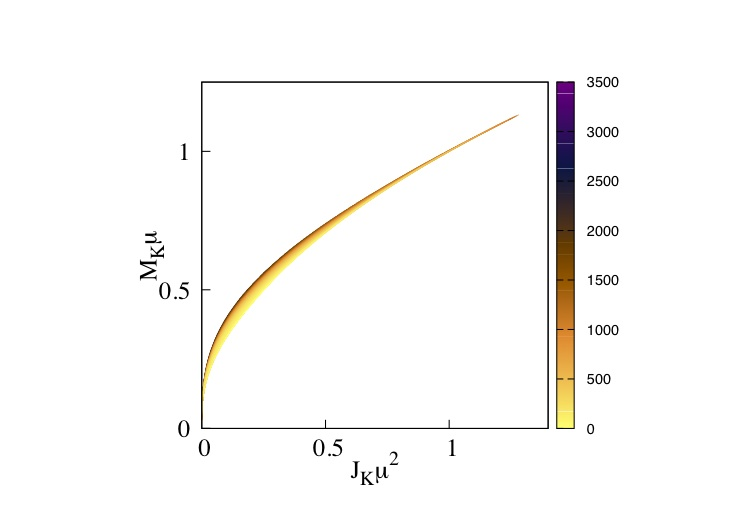
\includegraphics[height=2.15in]{papers/QClouds/EMJ-2D.jpeg}
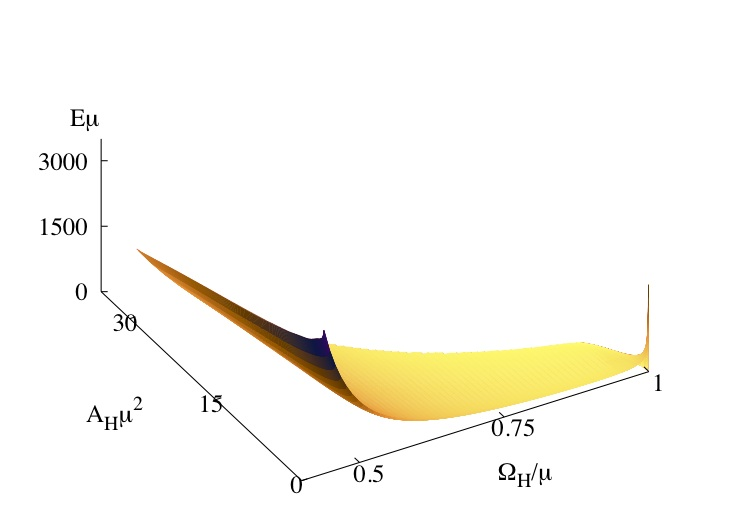
\includegraphics[height=2.15in]{papers/QClouds/EAHw-3D.jpeg}
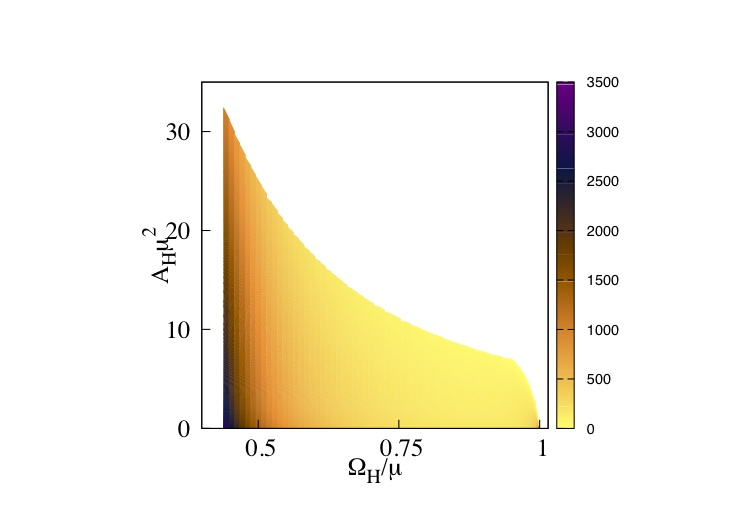
\includegraphics[height=2.15in]{papers/QClouds/EAHw-2D.jpeg}
\caption{$Q$-clouds energy, $E$, as a function three different combinations of parameters for the Kerr background, exhibited in both 3-dimensional (left panel) and 2-dimensional (right panel) plots: (top panel) mass $M_K$ and event horizon velocity $\Omega_H$; (middle panel) $M_K$ and angular momentum $J_K$; (lower panel) event horizon area $A_H$ and  $\Omega_H$.   
} 
\label{energy1}
\end{figure}

Similarly to the flat spacetime case,
  the study of the solutions with $w\to w_{min}$
  is rather difficult, since
 both the energy and angular momentum of the $Q$-clouds 
 take very large values in this limit. 
 At the same time, and in contrast to flat space $Q$-balls, the charges of $Q$-clouds
 remain finite as the maximal frequency is approached. In this case, the black hole background plays the role of a regulator.
 %
 These limiting behaviours are illustrated in Fig. \ref{spectrum}, where we plot the energy spectrum of $m=1$ $Q$-balls,
 $E(w)$,
 for several fixed values of the horizon area $A_H$.
 One can see that $Q$-clouds on a ``small''  Kerr black hole
 approach  for $w_{max}<\mu$,
 a critical configuration with zero global charges; this configuration sits 
 on the corresponding ($n=0,~l=m$)  existence line.
On the other hand, $Q$-clouds on a ``large'' Kerr black hole 
 end at a critical configuration with nonzero mass-energy and angular momentum;
 the corresponding Kerr backgrounds have $T_H=0$. 
 
 \begin{figure}[h!]
\centering
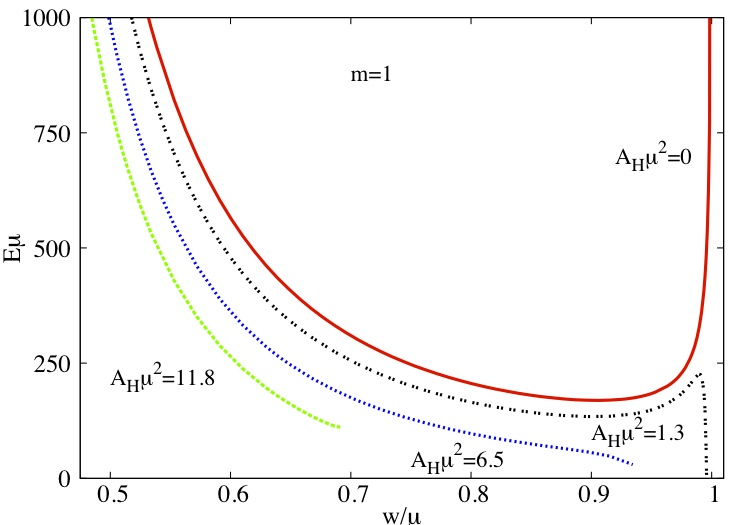
\includegraphics[height=2.8in]{papers/QClouds/Ew-fixed-AH.jpeg}
\caption{The spectrum of $Q$-clouds for several
fixed values of the event horizon area $A_H$.
The solutions with $A_H=0$
are the flat space $Q$-balls.} 
\label{spectrum}
\end{figure}
   
 
 
 %%%%%%%%%%%%%%%%%%%%%%%%%%%%%%%%%%%%%%%%%%%%%%%%%%%%%%%%%%%%%%%%%%%%%%%%%%%%%%%
\section{Further remarks} 
%%%%%%%%%%%%%%%%%%%%%%%%%%%%%%%%%%%%%%%%%%%%%%%%%%%%%%%%%%%%%%%%%%%%%%%%%%%%%%%

We have shown that
the well-known flat space $Q$-balls 
possess generalizations on a rotating black hole background -- $Q$-clouds. These bound states are 
in synchronous rotation with the black hole horizon, i.e. they obey condition (\ref{super_cond}).
Remarkably,
the self-interactions allow the existence of non-linear clouds 
in a \textit{2-dimensional} subspace of the full parameter space of Kerr black holes.
%
This subspace is bounded by the flat spacetime $Q$-balls,
the  $n=0,l=m$ existence line of linear clouds~\cite{Benone:2014ssa}
and a critical curve delimited by the minimal frequency of the scalar field.
 
The backreaction of $Q$-clouds leads to a new family of Kerr black holes with scalar hair in the full Einstein-scalar field system, when this type of self interactions are included. The new solutions have quantitative and qualitative differences, relatively to the Kerr black holes with scalar hair found in~\cite{Herdeiro:2014goa}. We have obtained some examples of these solutions, both for the self interactions studied here and another case.
This will be discussed at the end of Chapter \ref{ch:SI}.

Finally, let us mention that we have found no bound state solutions on the Kerr background for self-interacting scalar fields with the renormalizable potential $U(|\Phi|) =  \mu^2 |\Phi|^2+\lambda |\Phi|^4$.
However, as we will see in the next chapter, hairy black holes with such a potential do exist.
In a similar spirit,  boson stars can exist for this potential~\cite{Colpi:1986ye,Schunck:2003kk},  but they trivialize in the flat space limit, since the potential does not support $Q$-balls. 
